\section{Internal}\label{s:internal}

%-------------------------------------------------------------------------
\subsection{NVMeVirt}

\begin{comment}
NVMeVirt\cite{nvmevirt} is a Linux kernel module that provides a virtual NVMe device to the system, supporting various types of SSDs including basic SSDs, ZNS SSDs, and key-value SSDs.
The device is emulated at the PCI layer and can be used not only for standard devices but also for advanced storage configurations such as NVMe-over-Fabrics offloads.

The storage space of modern SSDs is divided into multiple partitions, as shown in Figure \ref{fig:structure}, with each partition managed by a separate FTL instance.
As a result, multiple FTL instances exist within a single SSD, sharing one PCIe link connected to the host.
Each partition consists of several NAND channels, and each channel is connected to multiple dies.
This architecture allows for data transfer through NAND channels to be serialized, while each die can operate independently.
In this structure, the FTL coordinates the dies and channels to handle I/O requests.
Thanks to this design, a single I/O request can be split into smaller tasks and distributed across multiple FTL instances, allowing for parallel processing.

As the data density per cell increases, the NAND programming time has also increased.
To hide this time, a write buffer is employed.
The data from incoming write requests is stored in the write buffer, and the write request is considered complete when the payload is copied to the write buffer.
If this write buffer becomes full, the data must be processed.
However, in NVMeVirt, to facilitate one-shot programming, this data is not immediately processed.
Instead, it waits until the buffering of another logical page in the same physical page is completed, after which the data is moved to the corresponding FTL for storage.
Once the write operation is complete, the FTL instance is reclaimed.
This processing occurs in the background.
For reads, the data is sent directly from the FTL instance to the buffer specified in the NVMe command without passing through the write buffer.

The storage of NVMeVirt is located in memory.
Since a significant amount of memory is required for data storage, it is necessary to reserve a portion of the physical address space at system initialization through boot parameters, as shown in Figure \ref{fig:making}.
Additionally, a simple linear mapping is used for data placement based on a conventional SSD.
Therefore, the memory location for the physical block and page numbers in the flash address space is calculated by adding the starting address of the reserved memory area.

There are several tools available for simulating or emulating SSDs.
Simulators use data processing models to mimic the internal operations of actual devices.
Their primary purpose is to construct models of the devices and parameterize the performance of internal operations to calculate desired performance metrics in the model.
As a result, while detailed analysis is possible, executing actual workloads can slow down the overall system when simulating the entire system.

Many emulators similar to NVMeVirt exist; for instance, FlexDrive can only emulate existing SSD types and does not support devices like KVSSDs and ZNS SSDs.
Our research aimed to reduce the time required for aging when conducting new studies, so we sought an emulator that could be used across various devices and thus did not utilize those emulators.
FEMU, on the other hand, provides a virtual NVMe device to guest operating systems by leveraging device virtualization features.
However, in a virtual machine environment, the guest physical memory is scattered across the host's physical memory through the host's virtual memory system, which can be inconvenient, and there is also the hassle of needing to reboot during experiments.

In contrast, NVMeVirt allows developers to easily modify the NVMe interface layer, enabling exploration of various design spaces and support for new device types.
Additionally, because it does not rely on virtualization technology, it permits comprehensive communication models with low overhead, and its modular design allows for easy usage through module loading.
For these reasons, we conducted our research on NVMeVirt.

Using an emulator like NVMeVirt enables direct access to the FTL, making our research feasible.
Through our research, we aim to facilitate the rapid creation of aged SSDs for future studies.
\end{comment}

% intro => What is NVMeVirt
% NVMeVirt는 소프트웨어로 정의된 NVMe 장치로, 리눅스 커널 모듈로 구현되어 있으며, 기존 NVMe 인터페이스를 사용하여 다양한 저장 장치를 모방하는 기능을 제공합니다.
% 주 목적은 고급 저장 장치를 개발하고 연구할 수 있는 환경을 제공하는 것으로, 실제 저장 장치와 유사한 방식으로 동작하게 됩니다.

As our idea is implemented using NVMeVirt~\cite{nvmevirt,empowering:tos23}, we first provide a brief overview of NVMeVirt internals.
NVMeVirt is a storage device emulator capable of presenting various NVMe device types.
Unlike other emulators, NVMeVirt emulates devices by processing NVMe commands at the PCIe level, thereby offering a flexible and realistic environment for evaluating diverse storage devices.
Currently, NVMeVirt supprots conventional SSDs, NVM SSDs, key-value SSDs, zoned namespace (ZNS) SSDs.


% development => How Work?
% NVMeVirt는 다양한 구성 요소로 이루어진 소프트웨어 정의 NVMe 장치로, 내부 구조는 FTL(Flash Translation Layer) 인스턴스, 채널, 다이(die), 블록, 페이지를 포함하여 데이터 처리를 수행합니다.
% PCIe 링크를 통해 직렬화된 데이터 전송에도 불구하고, FTL은 여러 NAND 채널과 다이를 통해 데이터 I/O 요청을 병렬로 처리합니다.
% 이러한 아키텍처에서 FTL은 다이와 채널을 조정하여 효율적인 데이터 처리를 진행하며, 각 다이는 독립적으로 작동하여 성능을 극대화합니다.

\begin{figure}[t]
    \centering
    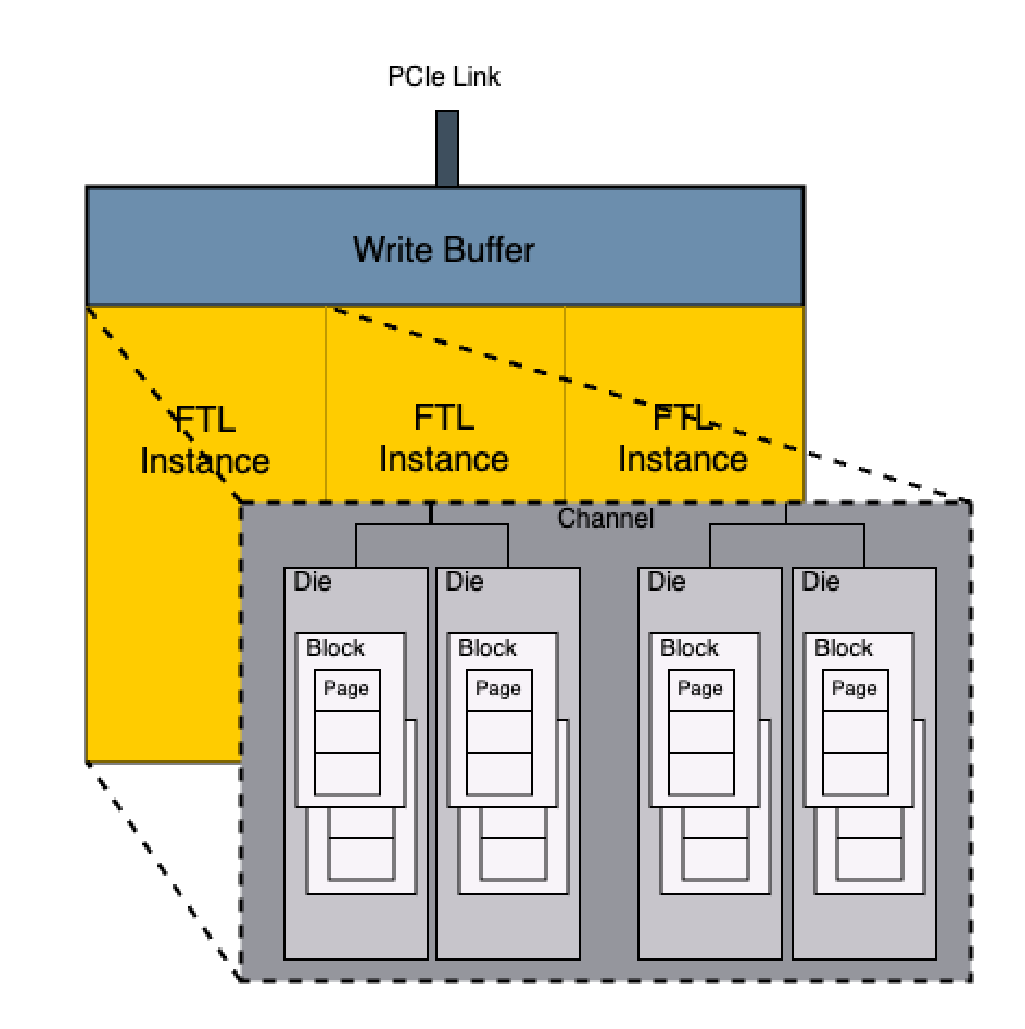
\includegraphics[width=0.95\columnwidth]{ssd}
    \caption{The internal architecture of NVMeVirt}
    \label{fig:structure}
\end{figure}

NVMeVirt is implemented as a Linux kernel module and consists of of several components.
The internal architecture is illustrated in Figure~\ref{fig:structure}.
To accurately reflect the inherent parallelism of modern SSDs, NVMeVirt is comprised of multiple FTL instances.
Each FTL instance takes charge of a part of LBA space, emulating the full hierarchy of core storage hardware components such as PCIe links, channels, dies, blocks, and pages.
NVMeVirt models realistic data processing by coordinating the abstraction of channels and dies.
Inbound data transferred over the PCIe link is first buffered in a write buffer, then dispatched to the appropriate FTL instance.
Each FTL instance handles I/O requests in parallel across multiple NAND channels and dies.


% 시스템 초기화 시 물리적 주소 공간의 일부를 예약하여 필요한 메모리를 확보하고, 이 예약된 메모리는 I/O 작업자, NVMeV 코어 디스패처 및 SSD 코어 등 NVMeVirt의 주요 구성 요소에 데이터를 저장하고 관리하는 데 사용됩니다.
% 사용자는 구성 파일을 통해 SSD의 종류를 지정하고 메모리의 시작과 끝 주소를 설정할 수 있어, 다채로운 구성 옵션을 선택택할 수 있습니다.

% 내부적으로 디스패처와 I/O 작업자가 상호작용하며 네이티브 NVMe 장치처럼 데이터를 처리합니다.
% 이러한 에뮬레이션 방식은 저장 장치 연구와 엔지니어링을 위한 다재다능함을 보여줍니다.
% 더불어 NVMeVirt는 다양한 저장 장치 유형인 일반 SSD, NVM SSD, ZNS SSD, 키-값 SSD를 지원하며, 다양한 저장 장치 인스턴스를 생성하여 연구자들이 여러 SSD 아키텍처를 실험하고 분석할 수 있는 기회를 제공합니다.

\begin{figure}[t]
    \centering
    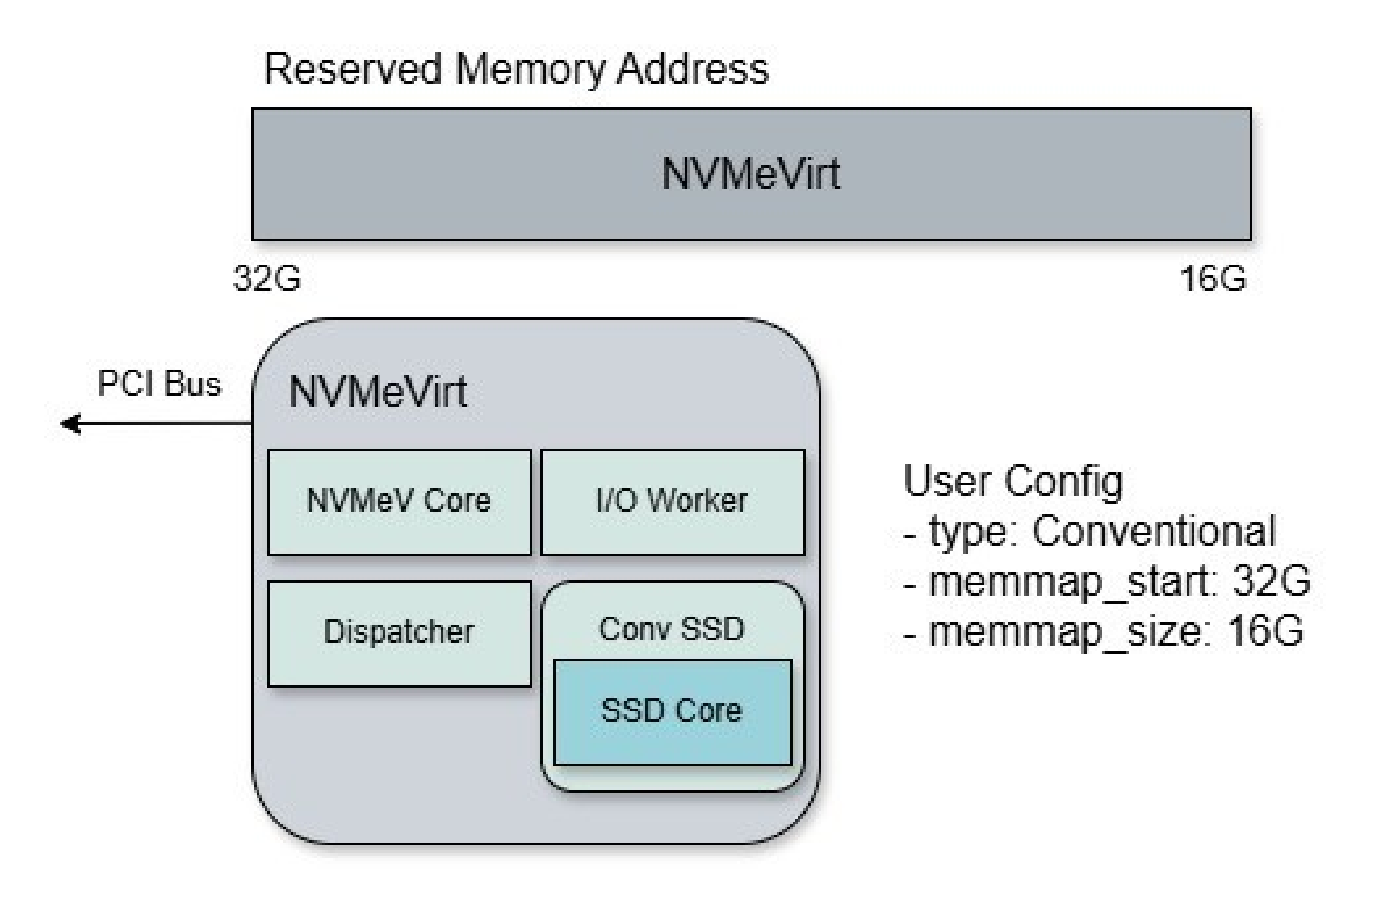
\includegraphics[width=0.95\columnwidth]{nvmev-making}
	\caption{Make the NVMeVirt instance\SK{그림이 뭘 이야기 하려는지 명확하지 않아요...}}
    \label{fig:making}
\end{figure}

% Initialization
Figure~\ref{fig:making} illustrates the process through which NVMeVirt instantiates virtual devices.
During system initialization, a portion of physical memory range is reserved.
The reserved memory can later be assigned to virtual devices during instantiation.
Users can create a device instance by specifying the device type and the memory range to assign via the sysfs interface.
The information is passed to the NVMeVirt module, which triggers a PCIe bus scan with an appropriate PCIe configuration header.
This process effectively create an instance of NVMe device of the specified type.
The device instance is visible to the system as if it is an actual device.


% Space
The assigned memory is utilized in a device type-specific manner.
For many device types, such as conventional SSDs, NVM SSDs, and ZNS SSDs, most of the reserved memory is used to store user data.
Specifically, a physical memory range is directly corresponds to the LBA space of the emulating device.
On top of the LBA space, each device type-specific FTL emulates the physical data layout, mapping LBNs to physical addresses.
During this process, the FTL models the device performance by computing the time required to complete each I/O request.

%This infrastructure enables researchers to instantiate multiple device instances, facilitating various evaluation environments.
%Internally, the dispatcher and I/O worker interact to process data like a native NVMe device.


\begin{comment}
% trun => Others

% SSD를 시뮬레이션하거나 에뮬레이션하기 위한 여러 도구는 이미 존재합니다.
% 시뮬레이터는 데이터 처리 모델을 사용하여 실제 장치의 내부 작업을 모방합니다.
% 이들의 주요 목적은 장치 모델을 구축하고 내부 작업의 성능을 매개변수화하여 모델에서 원하는 성능 메트릭을 계산하는 것입니다.
% 결과적으로, 상세한 분석이 가능하지만 전체 시스템을 시뮬레이션할 경우 실제 작업을 실행하는 데 시간이 지연될 수 있기 때문에 저희의 연구에서는 알맞지 않습니다.

% 에뮬레이터인 FlexDrive는 기존 SSD 유형만 에뮬레이션할 수 있고 KVSSD 및 ZNS SSD와 같은 장치는 지원하지 않습니다.
% 우리의 연구는 새로운 연구를 수행할 때 소요되는 노화 시간을 최소화하는 것을 목표로 하였기에, 다양한 장치에서 활용 가능한 에뮬레이터를 탐색하고자 하였습니다.
% 또 다른 에뮬레이터 장치 FEMU는 장치 가상화 기능을 활용하여 게스트 운영 체제에 가상 NVMe 장치를 제공합니다.
% 그러나 가상 머신 환경에서는 게스트 물리 메모리가 호스트의 가상 메모리 시스템을 통해 호스트의 물리 메모리에 분산되어 있어 불편할 수 있으며, 실험 중 재부팅이 필요하다는 번거로움이 있습니다.

Several tools already exist for simulating or emulating SSDs.
These simulators use data processing models to mimic the internal operations of actual devices.
Their main purpose is to build device models and parameterize the performance of internal operations to calculate the desired performance metrics from the models.
As a result, while detailed analysis is possible, simulating the entire system can introduce delays in executing actual tasks, making it unsuitable for our research.

The emulator FlexDrive can only emulate existing types of SSDs and does not support devices such as KVSSD and ZNS SSDs.
Since our research aimed to minimize the aging time required for conducting new studies, we sought to explore emulators that could be utilized across various devices.
Another emulator device, FEMU, leverages device virtualization to provide virtual NVMe devices to guest operating systems.
However, in a virtual machine environment, the guest physical memory is distributed across the host's physical memory via the host's virtual memory system, which can be inconvenient, and it also requires rebooting during experiments.

% conclusion => Advantages over others

% 반대로, NVMeVirt는 개발자가 NVMe 인터페이스 레이어를 손쉽게 수정할 수 있도록 하여 다양한 설계 공간을 탐색하고 새로운 장치 유형을 지원할 수 있는 유연성을 제공합니다.
% 또한, 가상화 기술에 의존하지 않기 때문에 낮은 오버헤드로 포괄적인 통신 모델을 구현할 수 있으며, 모듈식 설계를 통해 모듈 로딩이 용이합니다.
% 이러한 특성 덕분에 우리는 NVMeVirt를 기반으로 연구를 진행하게 되었습니다.
% 추가적으로, NVMeVirt를 활용함으로써 FTL에 직접 접근할 수 있는 부가적인 이점을 얻었습니다.

Conversely, NVMeVirt provides developers with the flexibility to easily modify the NVMe interface layer, allowing them to explore various design spaces and support new device types.
Additionally, by not relying on virtualization technology, it can implement a comprehensive communication model with low overhead, and the modular design facilitates easy module loading.
Thanks to these characteristics, we proceeded with our research based on NVMeVirt.
Furthermore, leveraging NVMeVirt offers the additional advantage of direct access to the FTL.
\end{comment}


%-------------------------------------------------------------------------
\subsection{Implementation}

\subsubsection{What to Bring}

\begin{figure*}[t]
    \centering
    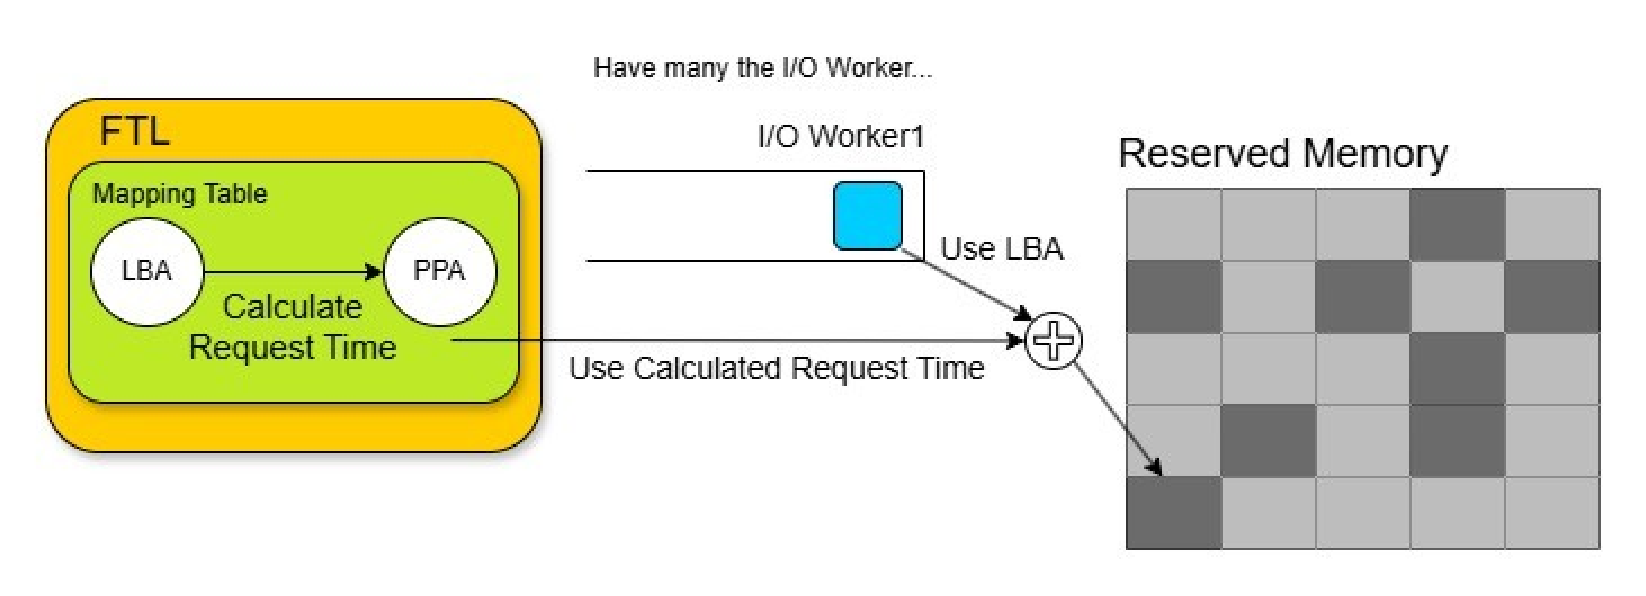
\includegraphics[width=0.95\textwidth]{mapping-table}
    \caption{NVMeVirt’s relation between FTL and data save process}
    \label{fig:mappingtable}
\end{figure*}

% Introduction
NVMeVirt emulates virtual devices entirely in software.
Our approach takes advantage of this by creating a snapshot of an aged device instance, which includes both user data and internal state information.
The Later, the instance can be fully restored by \emph{pouring} the snapshot into a newly created NVMeVirt instance, effectively recreating the aged state.
To enable this, four main types of data must be cpatured from the original instance to form a complete snapshot.


% 1. Mapping information
First, the \emph{mapping information} must be obtained.
Unlike actual SSDs, the FTL in NVMeVirt primarily performs the task of calculating request times.
When storing data in actual storage, it uses logical block addresses (LBAs) instead of physical page addresses (PPAs), eliminating the need to convert LBA to PPA for disk I/O assistance.
Instead, as shown in Figure \ref{fig:mappingtable}, the LBA is abstractly related to the PPA, and the expected request time is calculated so that the time taken to store or read data matches the computed request time.
This allows for abstract handling of each PPA.
Therefore, it is necessary to store the mapping table, reverse mapping table.


\begin{figure}[t]
    \centering
    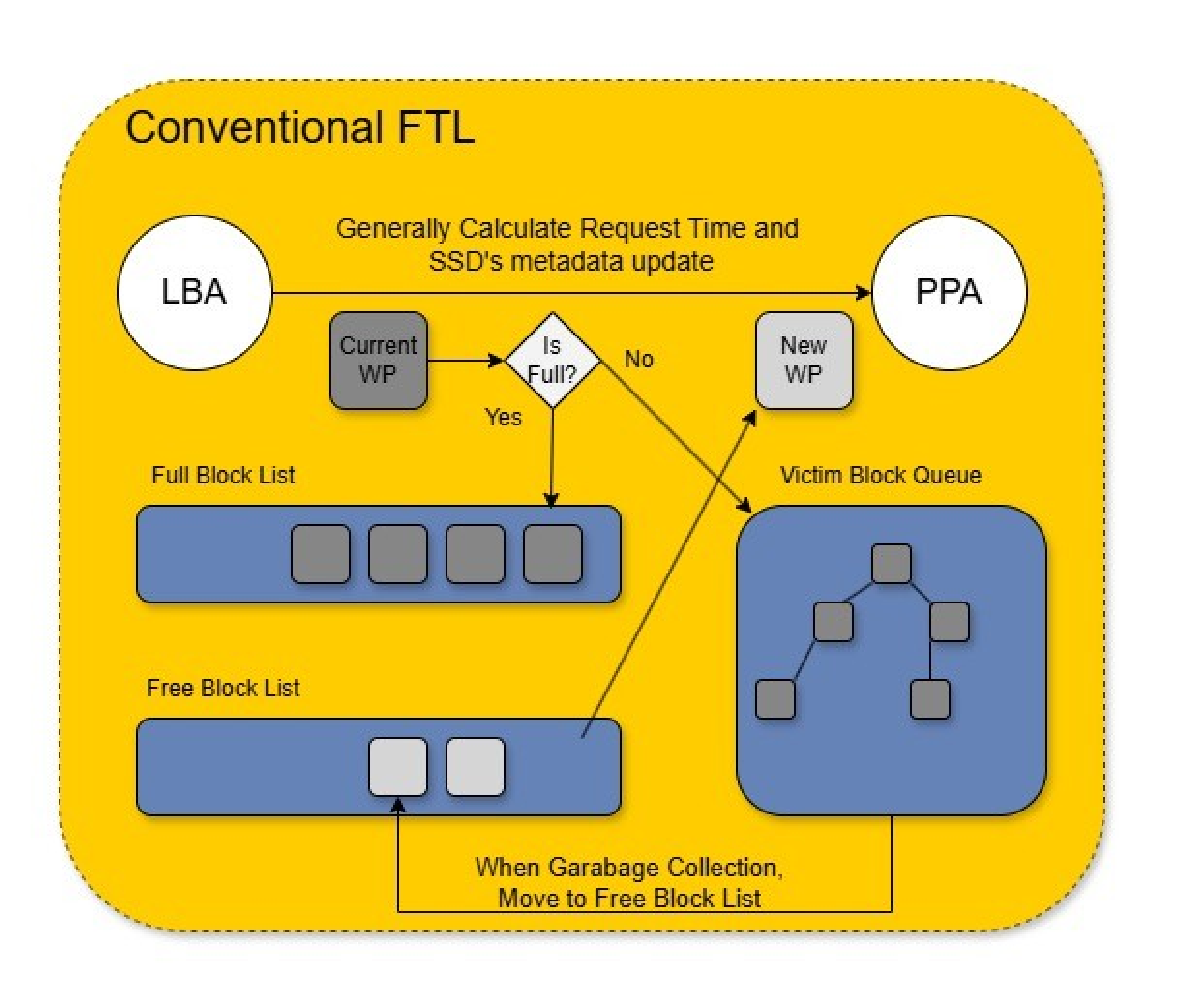
\includegraphics[width=0.95\columnwidth]{ftl-role}
    \caption{FTL’s role}
    \label{fig:role}
\end{figure}


% 2. Block metadata / block status
Second, we need to bring the \emph{Free Block list, Full Block list, and Victim Block queue} that manage the Free and Full blocks.
The state of an SSD's blocks is divided into two categories: Full Blocks, which are completely written, and Free Blocks, which are empty.
The FTL manages these blocks in list form.
As shown in Figure \ref{fig:role}, when the LBA is converted to PPA within the FTL and the request time is calculated, the write pointer is placed in either the Victim Block queue or the Full Block List.
The Victim Block queue contains blocks that have data written but are not yet in the Full Block state.
Later, through Garbage Collection, the data in these blocks is cleared to transition them to Free Block status.
The FTL manages Free Blocks through the Free Block List, allocating blocks from this list whenever a new write pointer is needed.
In other words, the state of the SSD blocks is managed through the Free Block List, Full Block List, and Victim Block queue, which determines where to write data.
Therefore, it is essential to preserve this data regarding block states.


% 3. SSD Metadata
Third, \emph{metadata about the SSD itself}, beyond the FTL, must be retrieved.
Since NVMeVirt is an emulator for SSDs, it manages metadata for channels, blocks, and pages.
Most of this data can be recreated in a new SSD without issues.
However, metadata for blocks and especially pages must be retained.
The page metadata includes the status of each page, which distinguishes whether the page is in a valid or invalid state.
When a new SSD is created, all pages are initialized to a valid state, so this information must be preserved.
For blocks, the metadata includes the count of valid pages, the count of invalid pages, and the erase count.
This information also needs to be maintained, as it will be reset in the new SSD.
Failing to retain the metadata for pages and blocks could lead to conflicts with the FTL's metadata, resulting in issues.

, and configuration parameters to calculate request times.


% 4. Contents
Lastly, the \emph{contents of the storage} must be retrieved.
The storage in NVMeVirt exists linearly in memory.
To obtain the contents of the storage, it is necessary to copy from the starting address of the storage for the entire size of the storage.


\subsubsection{Processing Save and Load}

% Introduction: we need to dump data
To maintain the data, it must be saved to external files and then loaded into the new SSD.
%
However, since NVMeVirt is a kernel module, this requires reading from and writing to files in user space from the kernel space.
Generally, reading and writing files from kernel space to user space is not recommended due to reasons such as kernel protection and over-reliance on User Space.
Nonetheless, in this research, the advantages gained from reading and writing files from kernel space outweigh the drawbacks, so we proceeded with this approach.

The data that needs to be preserved includes the FTL metadata, block lists, SSD storage metadata, and contents.
Instead of managing these in multiple files, we opted to store them in a single file for convenience in later distribution and SSD aging creation.
The functions used for reading and writing to the file are \cc{kernel\_write()} and \cc{kernel\_read()}.


% 1. block lists
There are two key points to highlight.
First is the block lists.
The FTL manages blocks in list form.
Since the mapping table is created as an array, the entire array can simply be copied.
However, for linked lists, this is not possible.
To copy a linked list, we must traverse the list and save the information in order.
Care must also be taken during loading; in the new SSD, all blocks exist in a Free Block state and are included in the Free Block List.
Even if multiple read and write operations have been conducted on the new SSD, the blocks included in the Free Block List and Full Block List will differ from those in the aged SSD.
Therefore, all lists must be initialized before loading.

% 2. data
The second point is the storage data saving process.
While the storage may contain contents across all ranges, it may also have empty spaces.
If we were to save the entire range of the storage to the file, it could include empty spaces, making it inefficient.
Thus, we aim to skip the empty spaces and only save the areas where data is present in the file.
This can be easily implemented using the mapping table.
The mapping table is stored in an array format, with the index representing the Logical Page Number (LPN) and the stored value representing the Physical Page Number (PPA).
NVMeVirt uses the LPN to store data in the storage and can verify whether data is stored in a given page using the PPA.
Therefore, by traversing the mapping table, we check whether data is stored in the page via the PPA, and if it is, we save the page's size to the file using the LPN.

% Loading
The loading process also utilizes the mapping table.
Similarly, since the data for the mapping table is saved and loaded together with the file, we can confirm the pages using the PPA and attempt to load the data into storage using the LPN.
This approach allows us to avoid storing unnecessary data, thereby reducing the file size for distribution and saving time.
